\chapter{ROS 2 Middleware Implementation for WebAssembly}

    The design of a custom middleware implementation, \textsf{rms-wasm}, that can be cross-compiled to WebAssembly modules is divided into three distinct packages as observed in Figure~\ref{fig:rmwwasm}. For this project, these packages were developed in the order shown, starting with \textsf{rmw-wasm-cpp}.

    \begin{figure}[htbp]
        \centering
        \vspace{1em}
        \begin{tikzpicture}
            \node (pkg) [
                rectangle,
                rounded corners,
                fill = shade05,
                text height = 7cm,
                align = justify,
                minimum width = 14cm,
                text width = 13.5cm,
            ] {\textsf{rmw-wasm}};

            \node (rwc) [
                packBox,
                yshift = 2.5cm,
                fill = shade15,
                ] {\textsf{rmw-wasm-cpp}};

            \node (wcpp) [
                packBox,
                yshift = 0.5cm,
                fill = shade15,
                ] {\textsf{wasm-cpp}};

            \node (wjs) [
                packBox,
                yshift = -2.5cm,
                fill = shade15,
                ] {\textsf{wasm-js}};
            
            \node (ems) [
                rectangle,
                yshift = -1cm,
                xshift = 2cm,
                ] {\texttt{emscripten::val}};

            \draw[thick] (rwc) -- (wcpp);
            \draw[thick] (wcpp) -- (wjs);

        \end{tikzpicture}
        \vspace{1em}
        \caption{Architecture of custom middleware implementation to target WebAssembly.}
        \label{fig:rmwwasm}
    \end{figure}

    \section{rmw-wasm-cpp}

        The first package, \textsf{rmw-wasm-cpp}, works as the ``adapter'' between \ac{ROS} 2 and the designed middleware. This package implements all of the functions required for \textsf{rmw} as described in Section~\ref{ssec:minimal}. The source code for this package is entirely written in C++ and can be found: TODO: 

        TODO: add diagram

        TODO: mention yaml conversion, add diagram?

    \section{wasm-cpp}

        The role of \textsf{wasm-cpp} is to implement the middleware and to function as a bridge to JavaScript modules. This package, along with \textsf{wasm-js} constitute the middleware implementation without the adapter, and thus, they can function independently of \textsf{rmw-wasm-cpp}. 

        The \ac{ROS} elements in this package build on top of each other, where the smallest unit is a \texttt{Participant}. Any \ac{ROS} subscriber, publisher, service server, service client, action server, or action client is simply a \texttt{Participant} with a specific role. Each \texttt{Participant} must have a valid name which follows the \ac{ROS} guidelines (TODO: add ref for valid names). For publishers and subscribers, this name is their respective topic name. And for servers and clients, the name corresponds to the service or action name.  Upon initialization, each \texttt{Participant} also receives a unique ID or \texttt{gid} which is used to keep track of individual participants. A class diagram illustrating the relations between the different elements is shown in Figure~\ref{fig:classes}.

        \begin{figure}[htbp]
            \centering
            \vspace{1em}
            \begin{tikzpicture}%[show background grid]
                \begin{abstractclass}[text width=5cm]{Participant}{0,0}
                    \attribute{- name : String}
                    \attribute{- role : String}
                    \attribute{- gid  : String}
    
                    \operation{- is\_valid\_name( )}
                    \operation{- is\_valid\_role( )}
                    \operation{- registration( )}
                    \operation{- deregistration( )}
                \end{abstractclass}
    
                \begin{class}[text width=5cm]{Publisher}{-5,-6}
                    \inherit{Participant}
                    \attribute{- name = topic\_name}
                    \attribute{- role = publisher}
                    \operation{+ publish(message : String)}
                \end{class}
    
                \begin{class}[text width=5cm]{Subscriber}{5,-6}
                    \inherit{Participant}
                    \attribute{- name = topic\_name}
                    \attribute{- role = subscriber}
                    \operation{+ get\_message( ) : String}
                \end{class}
    
                \begin{class}[text width=6.5cm]{ServiceServer}{-4,-11}
                    \inherit{Participant}
                    \attribute{- name = service\_name}
                    \attribute{- role = service\_server}
                    \operation{+ take\_request( ) : String}
                    \operation{+ send\_response(response : String)}
                \end{class}
    
                \composition{ServiceServer}{}{}{Publisher}
                \composition{ServiceServer}{}{}{Subscriber}
    
                \begin{class}[text width=6.5cm]{ServiceClient}{4,-11}
                    \inherit{Participant}
                    \attribute{- name = service\_name}
                    \attribute{- role = service\_client}
                    \operation{+ send\_request(request : String)}
                    \operation{+ take\_response( ) : String}
                    \operation{+ is\_service\_available( ) : Bool}
                \end{class}
    
                \composition{ServiceClient}{}{}{Publisher}
                \composition{ServiceClient}{}{}{Subscriber}
    
            \end{tikzpicture}
            \vspace{1em}
            \caption{A class diagram}
            \label{fig:classes}
        \end{figure}
        

        Subscribers and publishers are the simplest type of participants. And each of them only has one function; a publisher needs to be able to \textit{publish} a message, and a subscriber must be able to \textit{retrieve} the message from a specific topic. The messages which the publisher handles are yaml strings. These messages are then passed to \textsf{wasm-js} by using \texttt{emscripten::val} which transliterates JavaScript code into C++ (TODO: add ref). Figure~\ref{fig:publish} shows how these functions are implemented to create a \textit{bridge} between the two packages.

        \begin{figure}[htbp]
            \centering
            \begin{lstlisting}[language=C++]
// wasm_cpp/src/publisher.cpp
#include <emscripten/emscripten.h>
#include <emscripten/val.h>
...
emscripten::val js_publish = emscripten::val::module_property("publishMessage");
bool is_published = js_publish(yaml_message, topic_name).as<bool>();
\end{lstlisting}

            % To match syntax hightlight
            \begin{lstlisting}[language=C++] 
// wasm_js/src/pre.js
Module["publishMessage"] = function publishMessage(message, topic_name)
{
    if (message.startsWith("data:")) {
    self.postMessage({
        command: "publish",
        topic:    topic_name,
        message: message
    });
    }

    return true;
}
\end{lstlisting}
            \caption{Publisher sending a message to JavaScript for publishing.}
            \label{fig:publish}
        \end{figure}

    Conversely, the subscriber \textit{waits} for a response from \textsf{wasm-js} which will indicate that a new message has been published to the topic in question. The response message type is coerced into a yaml string to send back to \textsf{rmw-wasm-cpp}. This process is illustrated in Figure~\ref{fig:retrieve}.

    \begin{figure}[htbp]
        \centering
        \begin{lstlisting}[language=C++]
// wasm_cpp/src/subscriber.cpp
emscripten::val js_retrieve = emscripten::val::module_property("retrieveMessage");
emscripten::val js_response = js_retrieve(topic_name).await();
std::string yaml_message = js_response.as<std::string>();
\end{lstlisting}    
        \caption{Subscriber retrieving a message from JavaScript.}
        \label{fig:retrieve}
    \end{figure}

    With the configuration described, subscribers and publishers do not necessarily need to be aware of the existence of other participants within the same topic name. That is to say, a publisher can send messages even when there are no subscribers, and a subscriber can listen to a topic even when there are no messages published. Additionally, this allows multiple publishers to publish to the same topic simultaneously with different \ac{ROS} message types since all messages are handled as strings.

    Services are constructed from publishers and subscribers. A service server and a server client each have one publisher and one subscriber. Before a service client can call a service, it must verify that the service server is available to process a request. This is accomplished by making a query to \textsf{wasm-js} which keeps track of all available entities. If the service server is available, then the service client can \textit{publish} a request to the service request topic. Meanwhile, the service server is \textit{subscribed} to the service request topic to receive the request. Once the service server processes the request, the response tis \textit{published} to the service response topic. And lastly, the service client \textit{subscribed} to the response topic will retrieve the response. This process is summarized in Figure~\ref{fig:service}.

    \begin{figure}[htbp]
        \centering
        \vspace{1em}
        \begin{tikzpicture}
            \node (clt) [
                box,
                minimum width=3.5cm,
                text depth=3cm,
                xshift=-4cm,
                fill=shade20,
            ] {Service Client};

            \node (cltpub) [
                box,
                minimum width=3cm,
                minimum height=1cm,
                xshift=-4cm,
                yshift=0.5cm,
                fill=shade05,
            ] {Publisher};

            \node (cltsub) [
                box,
                minimum width=3cm,
                minimum height=1cm,
                xshift=-4cm,
                yshift=-1cm,
                fill=shade05,
            ] {Subscriber};

            \node (srv) [
                box,
                minimum width=3.5cm,
                text depth=3cm,
                xshift=4cm,
                fill=shade20,
            ] {Service Server};

            \node (srvsub) [
                box,
                minimum width=3cm,
                minimum height=1cm,
                xshift=4cm,
                yshift=0.5cm,
                fill=shade05,
            ] {Subscriber};

            \node (srvpub) [
                box,
                minimum width=3cm,
                minimum height=1cm,
                xshift=4cm,
                yshift=-1cm,
                fill=shade05,
            ] {Publisher};

            \node (t1) [
                box,
                minimum width=3cm,
                minimum height=1cm,
                yshift=0.5cm,
            ] {Request Topic};

            \node (t2) [
                box,
                minimum width=3cm,
                minimum height=1cm,
                yshift=-1cm,
            ] {Response Topic};

            \draw [arrow] (cltpub) -- (t1);
            \draw [arrow] (t1) -- (srvsub);
            \draw [arrow] (srvpub) -- (t2);
            \draw [arrow] (t2) -- (cltsub);

        \end{tikzpicture}
        \vspace{1em}
        \caption{Data flow between \ac{ROS} service client and server.}
        \label{fig:service}
    \end{figure}

    Analogously to services, action servers and clients are handled in the same manner with the addition that action servers will continuously publish feedback to the action response topic until the request being processed is completed.



%%%%%%%%%%%%%%%%%%%%%%%%%%%%%%%%%%%%%%%%%%%%%%%%%%%%%%%%%%%%%%%%%%%%%%%%%%%%%%%%

    \section{wasm-js}

        The last piece of the puzzle is \textsf{wasm-js}. This package is written in JavaScript and its role is to launch and track all the participating entities, and to store and distribute all \ac{ROS} messages accordingly.

        Given that processes on a browser run on a single ``main thread'', \textsf{wasm-js} uses \textit{web workers} to launch the requested \ac{ROS} nodes. Web workers run in background threads and thus, they do not interfere with the user interface while performing tasks~\cite{workers}. \textsf{wasm-js} spawns a new web worker for each \ac{ROS} node. The \ac{ROS} nodes can pass information to and from the main thread by posting messages (\texttt{postMessage()}). Each of the elements can also be configured to perform a task when a message is received by declaring an \texttt{onmessage()} function. Additionally, the workers can communicate between one another by creating message channels between worker pairs~\cite{mgschannel}. These communication paths are displayed in Figure~\ref{fig:webworker}.

        \begin{figure}[htbp]
            \centering
            \vspace{1em}
            \begin{tikzpicture}
                \node (thread) [
                    rectangle,
                    rounded corners,
                    minimum height = 1.5cm,
                    minimum width = \linewidth,
                    fill = shade20,
                ] {Main Thread};

                \node (w1) [
                    webBox,
                    xshift = -6cm,
                    yshift = -3cm,
                ] {ROS Node 1 \\ \footnotesize{web worker}};

                \node (w2) [
                    webBox,
                    xshift = -2cm,
                    yshift = -3cm,
                ] {ROS Node 2 \\ \footnotesize{web worker}};

                \node (w3) [
                    webBox,
                    xshift = 2cm,
                    yshift = -3cm,
                ] {ROS Node 3 \\ \footnotesize{web worker}};

                \node (w4) [
                    webBox,
                    xshift = 6cm,
                    yshift = -3cm,
                ] {ROS Node 4 \\ \footnotesize{web worker}};

                \node (post1) [
                    rectangle,
                    yshift = -1cm,
                    xshift = -3.5cm,
                ] {\texttt{postMessage()}};

                \node (post2) [
                    rectangle,
                    yshift = -2cm,
                    xshift = 3.5cm,
                ] {\texttt{postMessage()}};

                \node (onmsg1) [
                    rectangle,
                    yshift = -2cm,
                    xshift = -3.3cm,
                ] {\texttt{onmessage()}};

                \node (onmsg2) [
                    rectangle,
                    yshift = -1cm,
                    xshift = 3.3cm,
                ] {\texttt{onmessage()}};

                \node (chann) [
                    rectangle,
                    yshift = -4.5cm,
                    xshift = -2cm,
                ] {\texttt{MessageChannel()}};


                \draw [arrow, <->] (thread.south-|w1.north) -- (w1.north);
                \draw [arrow,  ->] (thread.south-|w2.north) -- (w2.north);
                \draw [arrow, <- ] (thread.south-|w3.north) -- (w3.north);
                \draw [arrow, <->] (thread.south-|w4.north) -- (w4.north);
                \draw [arrow, <->] (w1.south) -- + (0,-1) -| (w3.south);


            \end{tikzpicture}
            \vspace{1em}
            \caption{Communication between \ac{ROS} nodes as handled by \textsf{wasm-js}.}
            \label{fig:webworker}
        \end{figure}

        When the main thread receives messages from the web workers, it must not treat all messages equally. To accomplish this, each message contains a \textit{command} which tells the main thread how to process the information within. The commands are limited to the following options:

        \begin{itemize}
            \item \textbf{\texttt{register}}. A message with this command will also contain the name, the role, and the unique ID of a new participant to be added to the registration map.  
            \item \textbf{\texttt{deregister}}. This command type will provide the \texttt{gid} of the participant to be removed from the registration list; and in the case where this participant is also the last member of a topic or service, the message stacks for the particular topic or service will also be eliminated.
            \item \textbf{\texttt{publish}}. With this command, the message that the main thread receives will contain the \ac{ROS} message as a string and the name of the topic to be able to store the \ac{ROS} message in the correct message stack.
            \item \textbf{\texttt{retrieve}}. This command perform the opposite of publishing. The message data will contain the name of the topic where the most recent message should be retrieved to be able to select the message stack accordingly. And once the last \ac{ROS} message has been taken back and removed from the stack, the main thread will send this \ac{ROS} message back to the web worker which requested its retrieval.
            \item \textbf{\texttt{console}}. The message data sent with this command will include any errors, warnings, or simply output messages which would normally appear on a terminal. This helps make the information more accessible to the user.
        \end{itemize}

        To expand on how participants are added to the registration map; this map consists of multiple objects, where each object is responsible for storing all of the information relevant to a unique topic. Each object contains a list of ID's of topic members and a message stack. For services, two topic objects are created, one to store the information about service requests and the other to store service responses.

        

        \begin{figure}[htbp]
            \centering
            \vspace{1em}
            \begin{subfigure}[t]{0.32\textwidth}
                % 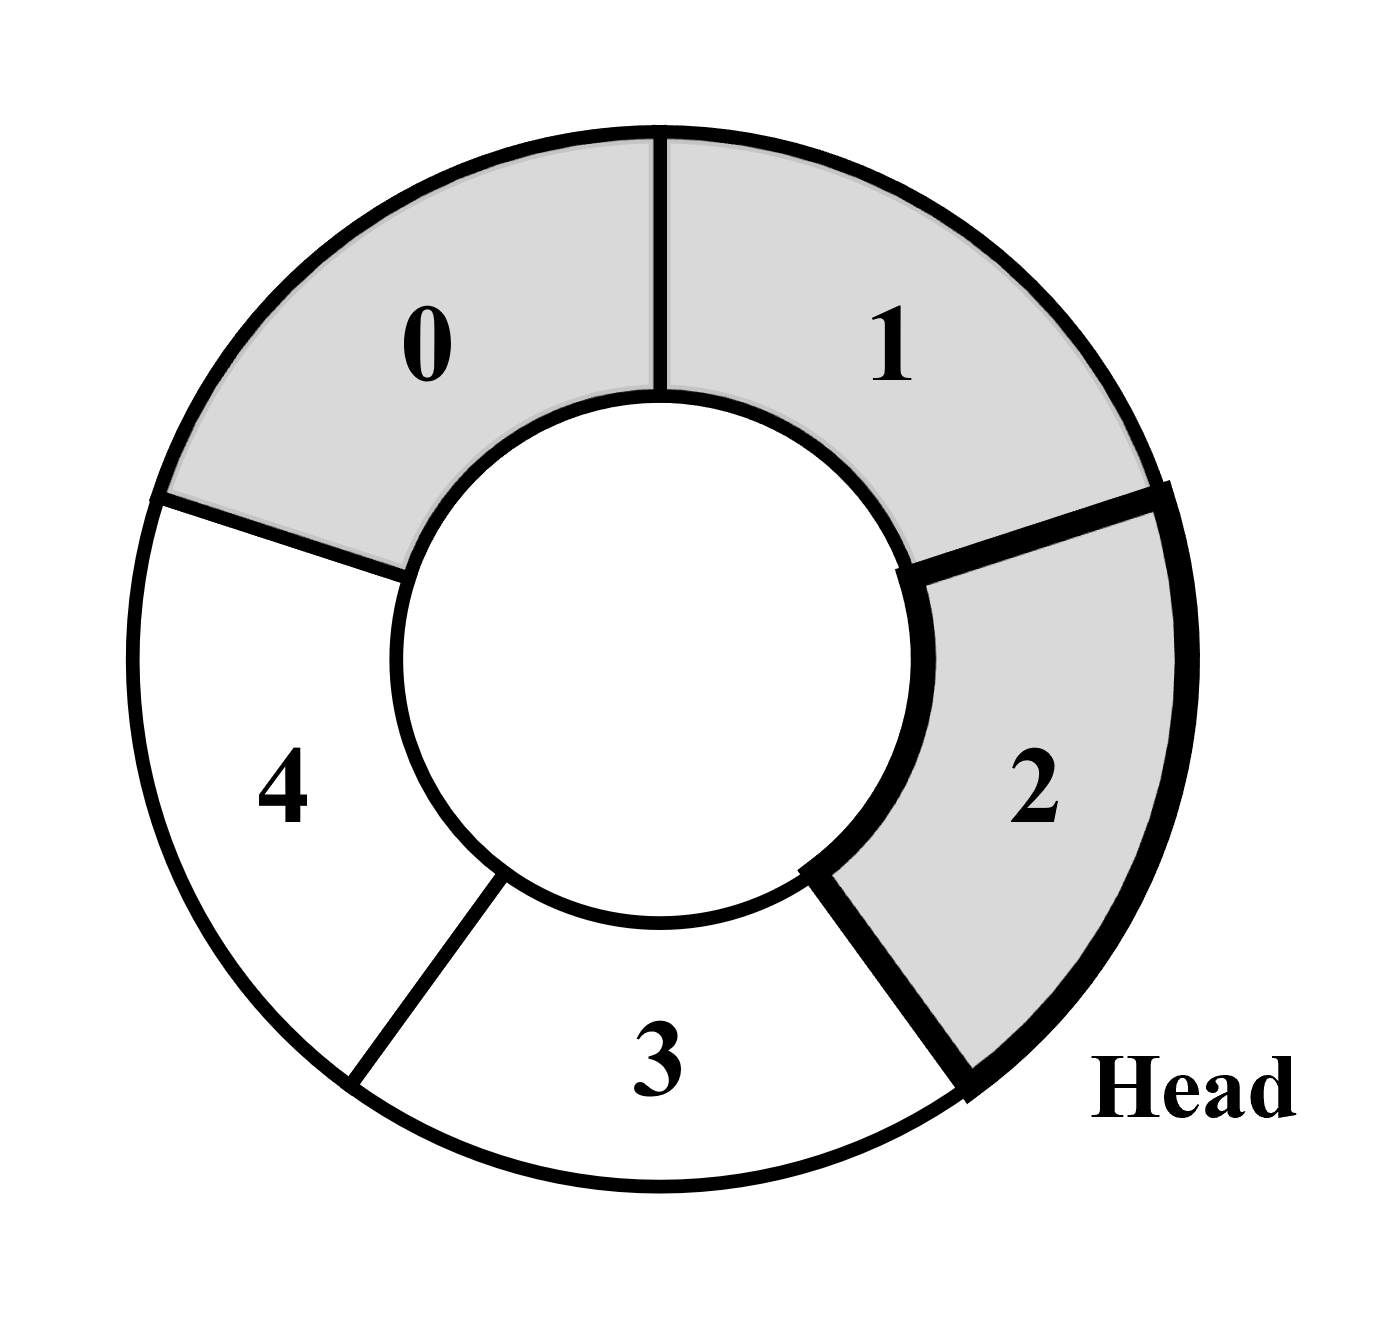
\includegraphics[height=0.9\textwidth]{07_stack0.png}
                \centering
                \begin{tikzpicture}
                    \node (m0) [
                        msg, 
                        fill = shade15
                    ] {\textbf{0}};
                    \node (m1) [
                        msg,
                        fill = shade15,
                        yshift = 1cm,
                    ] {\textbf{1}};
                    \node (m2) [
                        msg,
                        fill = shade15,
                        yshift = 2cm,
                    ] {\textbf{2}};
                    \node (m3) [
                        msg,
                        yshift = 3cm,
                    ] {\textbf{3}};
                    \node (m4) [
                        msg,
                        yshift = 4cm,
                    ] {\textbf{4}};
                    \node (head) [
                        rectangle,
                        yshift = 2cm,
                        xshift = 1.8cm
                    ] {Head};
                \end{tikzpicture}
                \caption{Filling stack}
            \end{subfigure}
            \begin{subfigure}[t]{0.32\textwidth}
                % 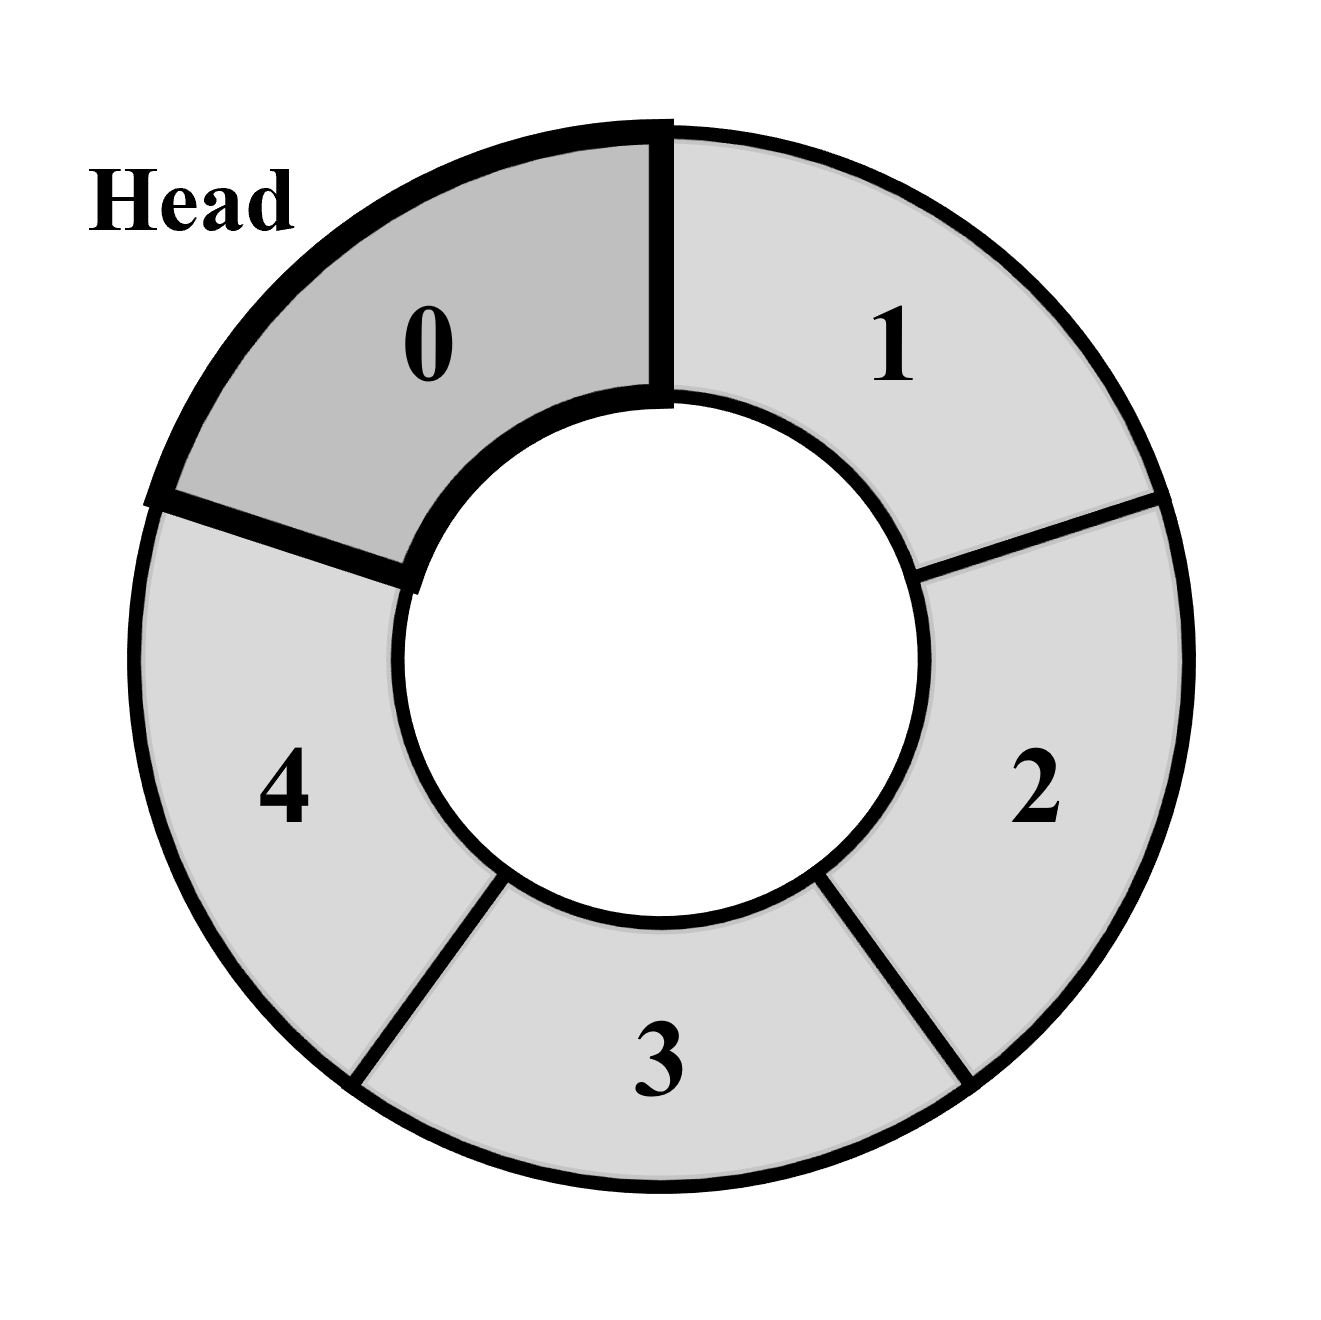
\includegraphics[height=0.9\textwidth]{07_stack1.png}
                \centering
                \begin{tikzpicture}
                    \node (m0) [
                        msg, 
                        fill = shade30,
                    ] {\textbf{0}};
                    \node (m1) [
                        msg,
                        fill = shade30,
                        yshift = 1cm,
                    ] {\textbf{1}};
                    \node (m2) [
                        msg,
                        fill = shade15,
                        yshift = 2cm,
                    ] {\textbf{2}};
                    \node (m3) [
                        msg,
                        fill = shade15,
                        yshift = 3cm,
                    ] {\textbf{3}};
                    \node (m4) [
                        msg,
                        fill = shade15,
                        yshift = 4cm,
                    ] {\textbf{4}};
                    \node (head) [
                        rectangle,
                        yshift = 1cm,
                        xshift = 1.8cm
                    ] {Head};

                    \draw [arrow] (m4.west) -- + (-0.5,0) |- (m0.west);
                \end{tikzpicture}
                \caption{Overwriting stack}
            \end{subfigure}
            \begin{subfigure}[t]{0.32\textwidth}
                % 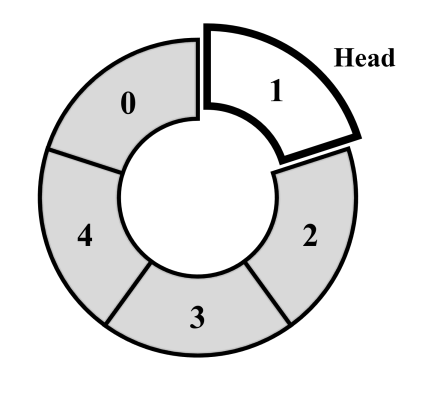
\includegraphics[height=0.9\textwidth]{07_stack2.png}
                \centering
                \begin{tikzpicture}
                    \node (m0) [
                        msg, 
                        fill = shade30,
                    ] {\textbf{0}};
                    \node (m1) [
                        msg,
                        yshift = 1cm,
                    ] {\textbf{1}};
                    \node (m2) [
                        msg,
                        fill = shade15,
                        yshift = 2cm,
                    ] {\textbf{2}};
                    \node (m3) [
                        msg,
                        fill = shade15,
                        yshift = 3cm,
                    ] {\textbf{3}};
                    \node (m4) [
                        msg,
                        fill = shade15,
                        yshift = 4cm,
                    ] {\textbf{4}};

                    \draw [arrow] (m1.east) -- + (0.5, 0);
                \end{tikzpicture}
                \caption{Reading stack}
            \end{subfigure}
            \vspace{1em}
            \caption{Modified Circular Stack, \ac{LIFO}}
            \label{fig:circleStack}
        \end{figure}


    - Message handling

